\documentclass[12pt]{article}

\usepackage[a4paper, total={7in, 9.5in}]{geometry}
\usepackage[english]{babel}
\usepackage{indentfirst}
\usepackage{fancyhdr}
\usepackage{setspace}
\usepackage{graphicx}
\usepackage{hyperref}
\usepackage{epsfig}
\usepackage{paralist}
\usepackage{lastpage}
% \usepackage[scaled]{helvet}
% \renewcommand\familydefault{\sfdefault}
\usepackage[T1]{fontenc}
\usepackage{url}
\usepackage{pgfplots}
\usepackage{tocbibind}
\usepackage{amsmath}
\usepackage{enumitem}
\usepackage{xcolor}

\pgfplotsset{compat=1.17}

\usepackage{xpatch}
\xpretocmd{\part}{\setcounter{section}{0}}{}{}

\pagestyle{fancy}
\fancyhf{}

\hypersetup{
  colorlinks=true,
  citecolor=blue,
  filecolor=black,
  linkcolor=blue,
  urlcolor=blue
}

\setlength{\parskip}{6pt}

\renewcommand{\headrulewidth}{0.3mm} % Top line width
\renewcommand{\footrulewidth}{0mm} % Bottom line width

\singlespacing

%Head
\lhead{\hspace*{0mm}\raisebox{3mm}{
  \epsfig{file=./logo/Aalto_en_1.pdf,height=11mm}}
}

\chead{\hspace*{50mm}\raisebox{7mm}{\hspace*{60mm}\small\begin{tabular}{r}
      \textbf{Programing Studio 2}\\CS-C2120\\\today\\
\end{tabular}}}

%Footer
\lfoot{}
\cfoot{}
\rfoot{\thepage}

\newcommand{\argmax}{\operatorname*{argmax}}
\newcommand{\argmin}{\operatorname*{argmin}}

\begin{document}

\begin{titlepage}
    \thispagestyle{fancy}
    \begin{center}
        \vspace*{1cm}
            
        \huge
        \textbf{Technical Plan}
            
        \vspace{0.5cm}
        \Large
        Balancer\\

        \normalsize
        \vspace{0.5cm}
        Final Project for CS-C2120
            
        \vspace{1.5cm}
            
        \textbf{Hau Phan}

        \normalsize
        886690
            
        \vfill

            
        Bachelor Degree in Science\\
        Data Science Program\\
        Years of study: 2020-2023
            
        \vspace{0.8cm}
            
        \normalsize
        Department of Computer Science\\
        Aalto University\\
        Finland, \today
    \end{center}
\end{titlepage}
\newpage

\tableofcontents
\addtocontents{toc}{\protect\hypertarget{toc}{}}
\newpage
\section{Class Structure}
\begin{figure}
  \centering
  \caption{UML Diagram for class structure}
  \vspace*{1cm}
  \hspace*{1cm}
  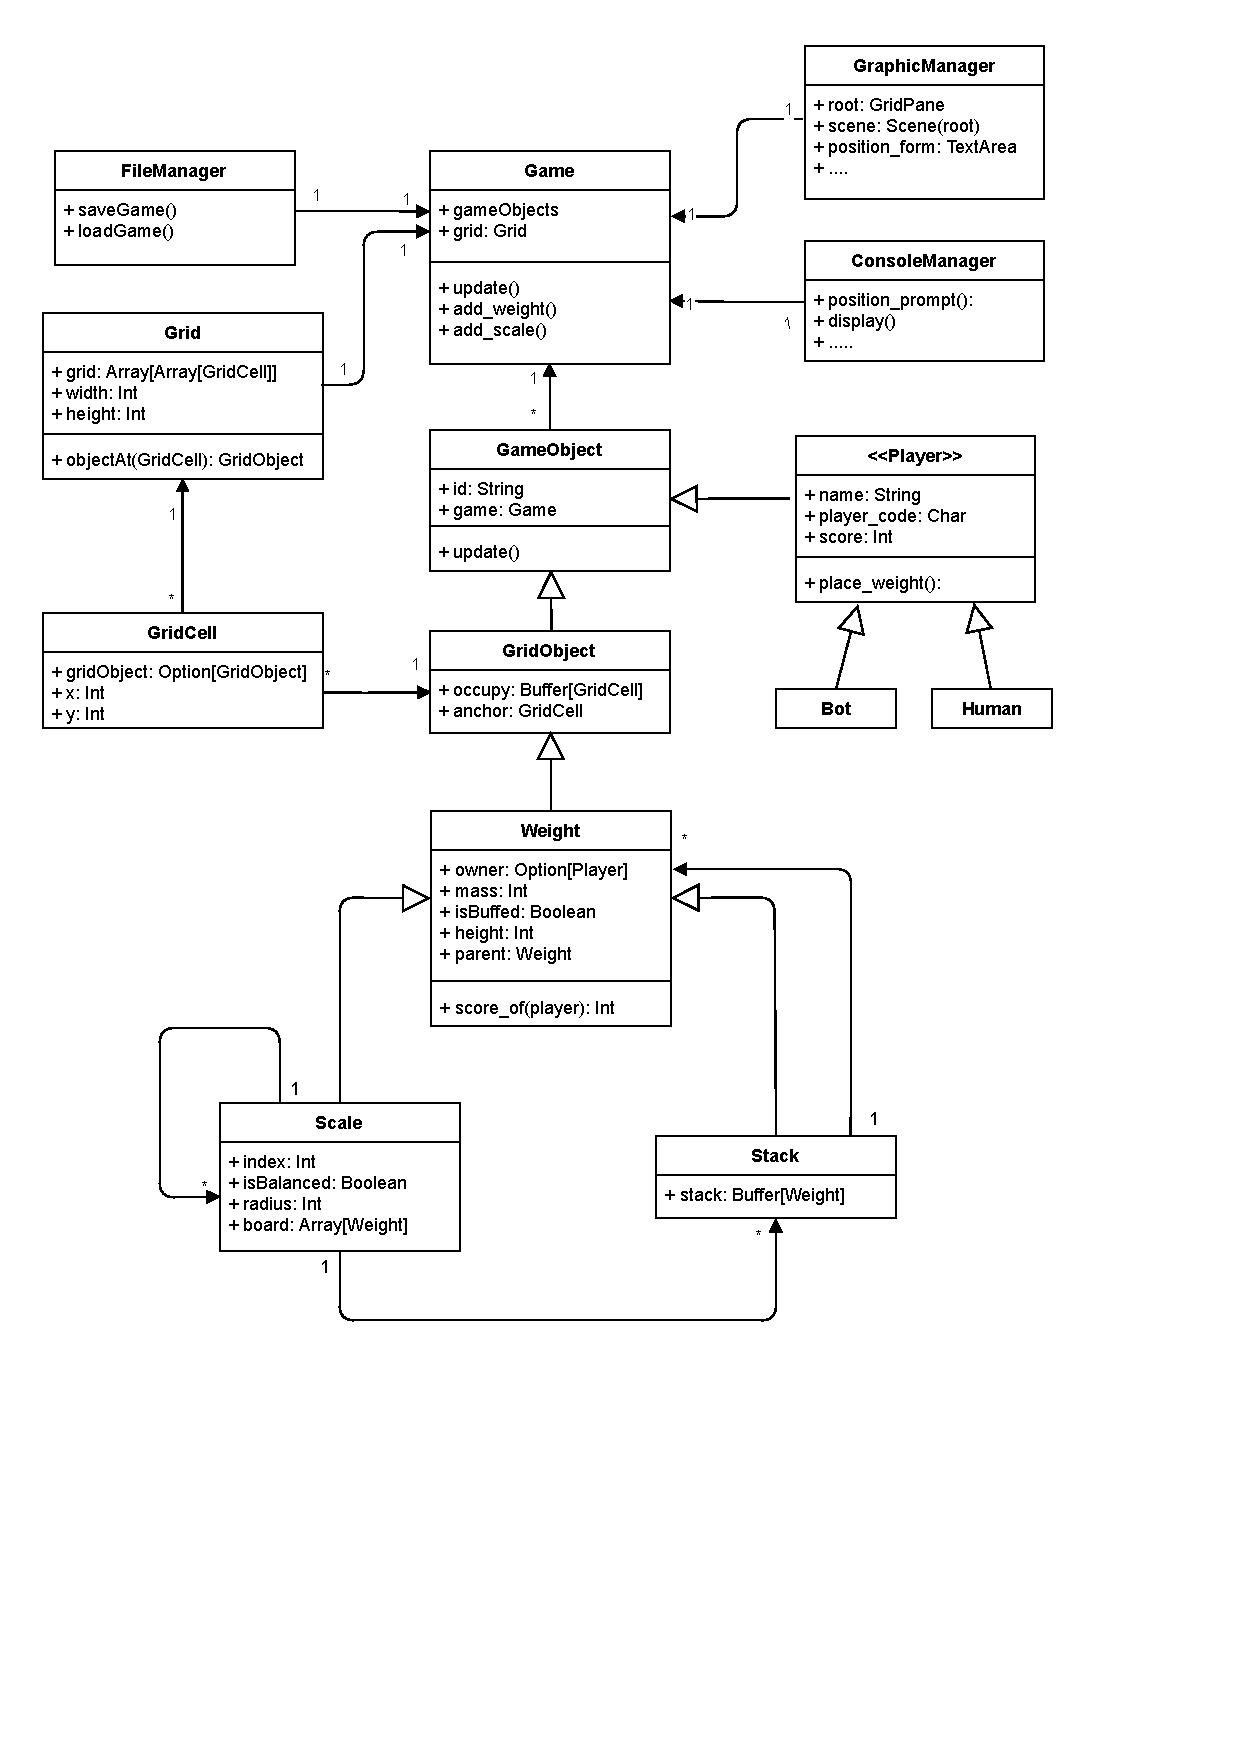
\includegraphics[width=\textwidth]{UML Project.pdf}
\end{figure}
\subsection{Game and GameObject}
The Game class will store the game state (players, scales, weights, \dots) in
the a hash map \textbf{gameObjects}. It also have a FileManager that manage the
process of saving and loading game state from a file.

\subsection{Player}
Player is a \textbf{sealed abstract} class which models a player in the game,
with two \textbf{case class} \textit{Bot} and \textit{Human}. 

The \textit{player\_code} attribute is a character (ex. "a", "b", "c", ....)
that represents player's weights in the text-based version of the game.  The
\textbf{score} attribute will be dynamically calculated.

\subsection{Grid, GridCell and GridObject}
The game objects, i.e weights and scales, are displayed on a grid. There is a
grid instance in the Game class and this will be interpreted by different
renderer (\textit{GraphicManager} and \textit{ConsoleManager}) to be display on
the screen. 

Each weight occupies only 1 GridCell while each scale occupies many. 

Each GridObject has a buffer that contains all the GridCell that they lie upon.
GridObject also has an anchor that signify the center of the shape. For a weight,
it just the single cell that it occupies, for a scale, it is the center of the
board.
\subsection{Weight, Scale and Stack}
The classes Weight, Stack, Scale model a single weight, a stack of weights and a
scale respectively. Stack and Scale is derived from Weight, thus they also have
an owner, mass and height. \textit{(Noted: height is only used in the algorithm
displaying these objects on the grid)}

The base Weight class and its derived classes Stack and Scale also have the
\textbf{parent} attribute, which store a reference to its parent.

\subsection{GraphicManager and ConsoleManager}
These two class will interpret the grid in the Game class and display it to the user,
graphically in a window or text-only on the console. 

GraphicManager also has UI elements such as TextArea and Button to prompt for
user input using ScalaFx. Both will update the game state by adding weight to
the gameObjects hash map. 

"Core" functions in the Game class such as \textit{add\_weight} and
\textit{add\_scale} will be used to automate this process.

\section{Use Case Description}

\subsection{Graphical}

The game starts and presents the \textbf{Menu scene} on the window, where
user(s) can use their mouse to click on one of three button: "Start new game",
"Load saved game", or "Quit" \textit{(Notes: a "Setting" button and "Setting
  Scene" might be added, where users can modify the configuration
file graphically)}

Clicking one of the three button will trigger the GraphicManager to switch to a
different scenes.
\subsubsection{Start New Game}

Clicking the "Start new game" button will lead to the \textbf{Setup Scene} being
shown where user(s) will first enter the number of players, then one at the
time, a pop-up form will show up asking for each user's name, and a tick box to
determine whether this player is a bot or not. This is handled by the
GraphicManager. When finished, user(s) will be shown the \textbf{Game Scene}
where user(s) spends most of the time interacting with the game. The
\textbf{Game Scene} was the drafted user interface in the General Plan of this
project:

\includegraphics[width=\textwidth]{Graphical User Interface.png}

The left gray region is where the player can move around, zoom in and out to
see which scales and weights is owned by whom and how they are placed. This
will be handled by a \textbf{Camera} and the GraphicManager.

The right white region is the main UI. The top part is the score board where
more information about the current state of the game is shown, for example each
player's score, the number of weights left,\dots. The information/text in ther
scoreboard will be binded directly to the game state and will update immediately
when the game state changes. The middle part is a form where player in his/her
turn can fill in and trigger the game to place the weight accordingly. The "End
turn" button will "call back" to the \textit{place\_weight()} in the Player
class to place the weight.

At the end of the round, a pop-up will be shown and announce the round's winner.
The game then continues to the next round, randomly placing some weights and a
scale. If there is no round left, a pop-up will announce the game 's winner
instead.


\subsubsection{Load Saved Game}

User(s) can also load previous state of the game from a saved file by clicking
the "Load Saved Game" button. The structure of the saved file is detailed in the
File and Format Section of the General Plan. Handling saving and loading game
state from file is done by the FileManager class, separated from main Game
class.

The "Quit" button simply ends the program.

\subsection{Text-on-console}

The program can be run on the command line with no parameter to start a new game
or with a path to the save file to resume previous games. \textit{Notes: This
might change in the future where user can pick in the game instead}

\subsubsection{New Game}

When a brand new game starts, it will prompt the user to enter some basic
information about the players, e.g, how many of them are there, their names,
\dots. Then the first round starts and each player will one at a time be
prompted for information on where his/her weight should be placed. The current
score of each players, the state of the game will also be shown to each players
for them to make a decision.

When a round finished, the winner of that round will be
announced. At the end of the game, the overall winner will be announced instead.

\subsubsection{Load Game}

When the save file is loaded successfully, the game will continue from the state
when it is saved. Otherwise, it will print out the line causing the failure and
exit.
\section{Algorithms}
Most components in the game requires some forms of algorithm/recursion and
mathematics to achieve its functionality:
\begin{itemize}
  \item Mass of an object the \textit{mass} attribute will be called recursively,
    summing the mass of all the objects it contains.
  \item Height of an object: the \textit{height} attribute of a scale will be
    called recursively, which is the \textbf{max} height of all the scales and
    stacks it contains. For a stack, it just the number of its weights.
  \item Checking whether the scale is balance: After having the mass of all the
    objects on the parent scale, we can calculate its imbalance. The formula is
    as follow:
    \begin{align*}
      Imbalance = \sum_{i=-r}^{r}i\;m_i
    \end{align*}
    where $r$ is the radius of the scale, $m_i$ is the mass of the object at
    distance $|i|$ from the center. Negative value of $i$ indicates the object
    is on the left arm of the scale.
  \item Score of a player: the score of player $p$ on an \textbf{object} $o$
    is a recursive piecewise function conditioned by $o$ and $p$:
    \begin{equation*}
      s(o,p) = \begin{cases}
        s(o, p) = \sum_{i=-r}^{r} |i|\;s(o_i, p) , &\text{ if $o$ is a scale}\\
        s(o, p) = \sum_{w\in S} s(w, p) , &\text{ if $o$ is a stack, with
        weights $S$}\\
        s(o, p) = 1 &\text{ if $o$ is a weight owned by $p$}\\
        s(o, p) = 0 &\text{ if $o$ is a weight not owned by $p$}
      \end{cases}
    \end{equation*}
    where $o_i$ is the object at distance $|i|$ from the center the scale.
    Negative value of $i$ indicates the object is on the left arm.
  \item Intelligent bot: the bot will use a recursive algorithm to traverse each
    scale, searching for all possible best moves that maximize its score gain in
    its turn and randomly picks one (or if there is only one best move, picked
    it).  \textit{Notes: Computing time is nearly instant for most game with
    human players, which should be at most 5-6 scales per round.} 
\end{itemize}
\section{Data Structures}

The \textbf{gameObjects} will server as an indexer/register for all GameObject
instances, whether it is a player, scale, stack or weight. It will be used
frequently to retrieve instances of GameObject by their unique ID. Therefore, it
will be implemented as a \textbf{HashMap or Map}, which has constant access and
insert time.

The grid object in the class Grid will be implemented as a 2D array of GridCell,
which has constant access and insert time, allowing for quick rendering of
objects. Implementing a grid as a 2D array also help in development since it is
easier to work with intuitively and have some programming caveats.

The Stack will be modeled as a Buffer, since it provides much of the
functionality and will be mutated frequently. \textit{Notes: While Scala's
collection package does have an implementation of an actual stack, Buffer is
used instead due to its familiarity and reliability.} 

The \textbf{board} of a Scale will be modeled as an Array because its length is
constant i.e the scale can not shrink or grow in length. Constant access speed
is also one reason to choose Array over Buffer for the \textbf{board}.


\section{Schedule}

The program can be divided into different areas/sections, grouped by its
role/concept that needed to be built, tested and documented. Here we also
introduce the concept of \textbf{"core"} classes and objects, parts of the
program that many other objects depend on them. In this project, they are the
main Game class, Weigh-Scale-Stack classes and the Player class. These
represents the fundamental ideas of the game and with them, gameplay is
achieved. Other classes will be build on top of them to either adding additional
functionality like save/load file or display them to the user either in a
graphical UI or on the console.

Different areas/sections will require different amount of time to go through the
3 phase mentioned above (built, test, document), with the core classes and the
UI being the most demanding ones. 

\begin{itemize}
  \item  The first two weeks (\textbf{22.2} - 7.3) will be dedicated to build
    and test different functionalities of these core classes. The bot algorithm
    may or may not be implemented in this period since it is not immediately
    essential and can be separated.
  \item The week after (8.3 - 14.3) will be dedicated to implement and test the
    save/load file functionality of the game. This will be important for testing
    the UI and the bot algorithm since generating test case will be much easier.
    Noted that the first interim report is due on 17.3.
  \item  The next 2.5 weeks (15.3 - 31.3) will be dedicated to build and test
    the UI for the game, on the console and graphically in a window. Noted: the
    second interim report is due on 31.3.
  \item  The next two weeks (1.4 -  14.4) will be dedicated to system testing of
    the whole program, debugging, tuning, optimizing for performance and adding
    additional features where needed. The final interim report is also due at
    the end of this period, on 14.4.
  \item  The final two weeks (14.4 - \textbf{28.4}) will be dedicated to writing
    the required documentation and act as a "buffer zone" if more time is needed
    to complete certain features.
\end{itemize}
\section{Testing}
\subsection{System testing}

For most functionalities and features, the program will be tested manually by
typing onto the console (for text-only version) or interacting with the
graphical UI directly (in a graphical window). The UI and the display of game
state will be manually tested for the most part with some aspect of the testing
will be automated if needed. Saving/loading game state and testing will be
frequently used in tandem.  The saved game file will be designed and modified
accordingly depending on which aspect of the game is being tested.

The goal for system testing is to minimize the chance of having bugs and
glitches in the final product and of course, verify that the game did what it
supposes to do and all its functionalities work correctly. System testing will
also assess other aspect of the program, for example, its user experience: is it
intuitive enough that anyone can pick up and use ?  Is the game good at
communicating its information to the user? etc \dots.

The test might be checking:
\begin{itemize}
  \item The weight is placed at the correct location according to the user
    inputs.
  \item All the information of the game such as the score, the round number, the
    number of weights, etc \dots is displayed correctly.
  \item The canvas displays the current state of the game and update
    when a new weight is placed.
  \item \dots
\end{itemize}

\subsection{Unit testing}

Individual component and function in the program will also be tested the during
implementation of the project. This is done to catch bugs and exceptions
immediately when coding and not later when testing other part of the program.
However, not all components and methods will need test case designed for them.
Simple "get", "set" and "short 1 liners" method will not be unit-tested. 

Some important "core" methods which are used frequently through out the program
might have "edge cases" and exceptions that only show up when implementing other
components, when they are linked together. This is tested during integration
testing.

Example of these "core" methods is \textit{add\_weight()} and
\textit{add\_scale()} in class Game, which will have multiple test case designed
for them, testing for different exceptions arose from invalid user inputs. Some
of the test for these might include testing for appropriate handling of
exceptions, for example, when an invalid position is chosen by the users.  For
\textit{add\_weight()}, it is when the location has already been occupied by a
scale or is outside the scale altogether. Or for \textit{add\_scale()} , it is
when there is a stack or scale already occupied the space.

Beside "core" methods, algorithms will also be tested frequently for accuracy
and return values. The two algorithms that will be tested extensively is the
bot's search algorithm for maximum score gain and the rendering algorithm for
GridObject and Grid. The test cases will be written in the saved file format to
represents different scenarios that the algorithm must either search for best
move or render onto the screen.

\nocite{nystrom2014game}
\nocite{scalacollection}
\bibliographystyle{unsrt}
\bibliography{/home/phanth/Academia/TEX-Latex/bib.bib}
\end{document}
